\documentclass[14pt]{beamer}

% Presento style file
\usepackage{config/presento}

\usepackage{booktabs}
%\usepackage[scale=2]{ccicons}
%\usepackage{minted}
%\usepackage{media9}
\usepackage{multimedia}
\usepackage{animate,media9}

% custom command and packages
% custom packages
\usepackage{textpos}
\setlength{\TPHorizModule}{1cm}
\setlength{\TPVertModule}{1cm}

\newcommand\crule[1][black]{\textcolor{#1}{\rule{2cm}{2cm}}}



\setbeamerfont{caption}{size=\scriptsize}

% number four:
\title{\large Quantitative characterization of endothelial cell polarity}
\subtitle{\small Automated segmentation, image data features extraction, statitistical analysis }

\author{\small ...}
\institute{MDC Berlin}


\begin{document}

% Title page
\begin{frame}[plain]
\maketitle
\centering

\end{frame}

\begin{frame}[plain]
\frametitle{\normalsize \bf Flow migration coupling}

\centering


\begin{figure}
  \centering
  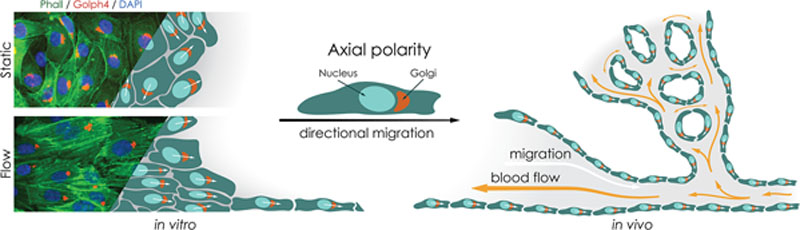
\includegraphics[width=0.9\textwidth]{images/leducq_attract.jpg}\\
  \tiny
   \textit{``Arterial Flow as Attractor for Endothelial Cell Migration``, Petya B. Georgieva, Douglas A. Marchuk, Holger Gerhardt, and Leducq ATTRACT Consortium, Circulation Research (2019).}
\end{figure}



\tiny

\begin{itemize}
 \item (1) flow migration coupling: blood flow induces wall shear stress (WSS), endothelial cells are assumed to orient against flow and migrate agains the WSS gradient
 \item (2) in static images the nuclei-golgi vectors are frequently used as a read-out for endothelial cell polarity \textit{in vivo} and \textit{in vitro}
\end{itemize}


\end{frame}


\begin{frame}[plain]
\frametitle{\normalsize \bf Segmentation with Cellpose}


\tiny
\begin{figure}
  \centering
  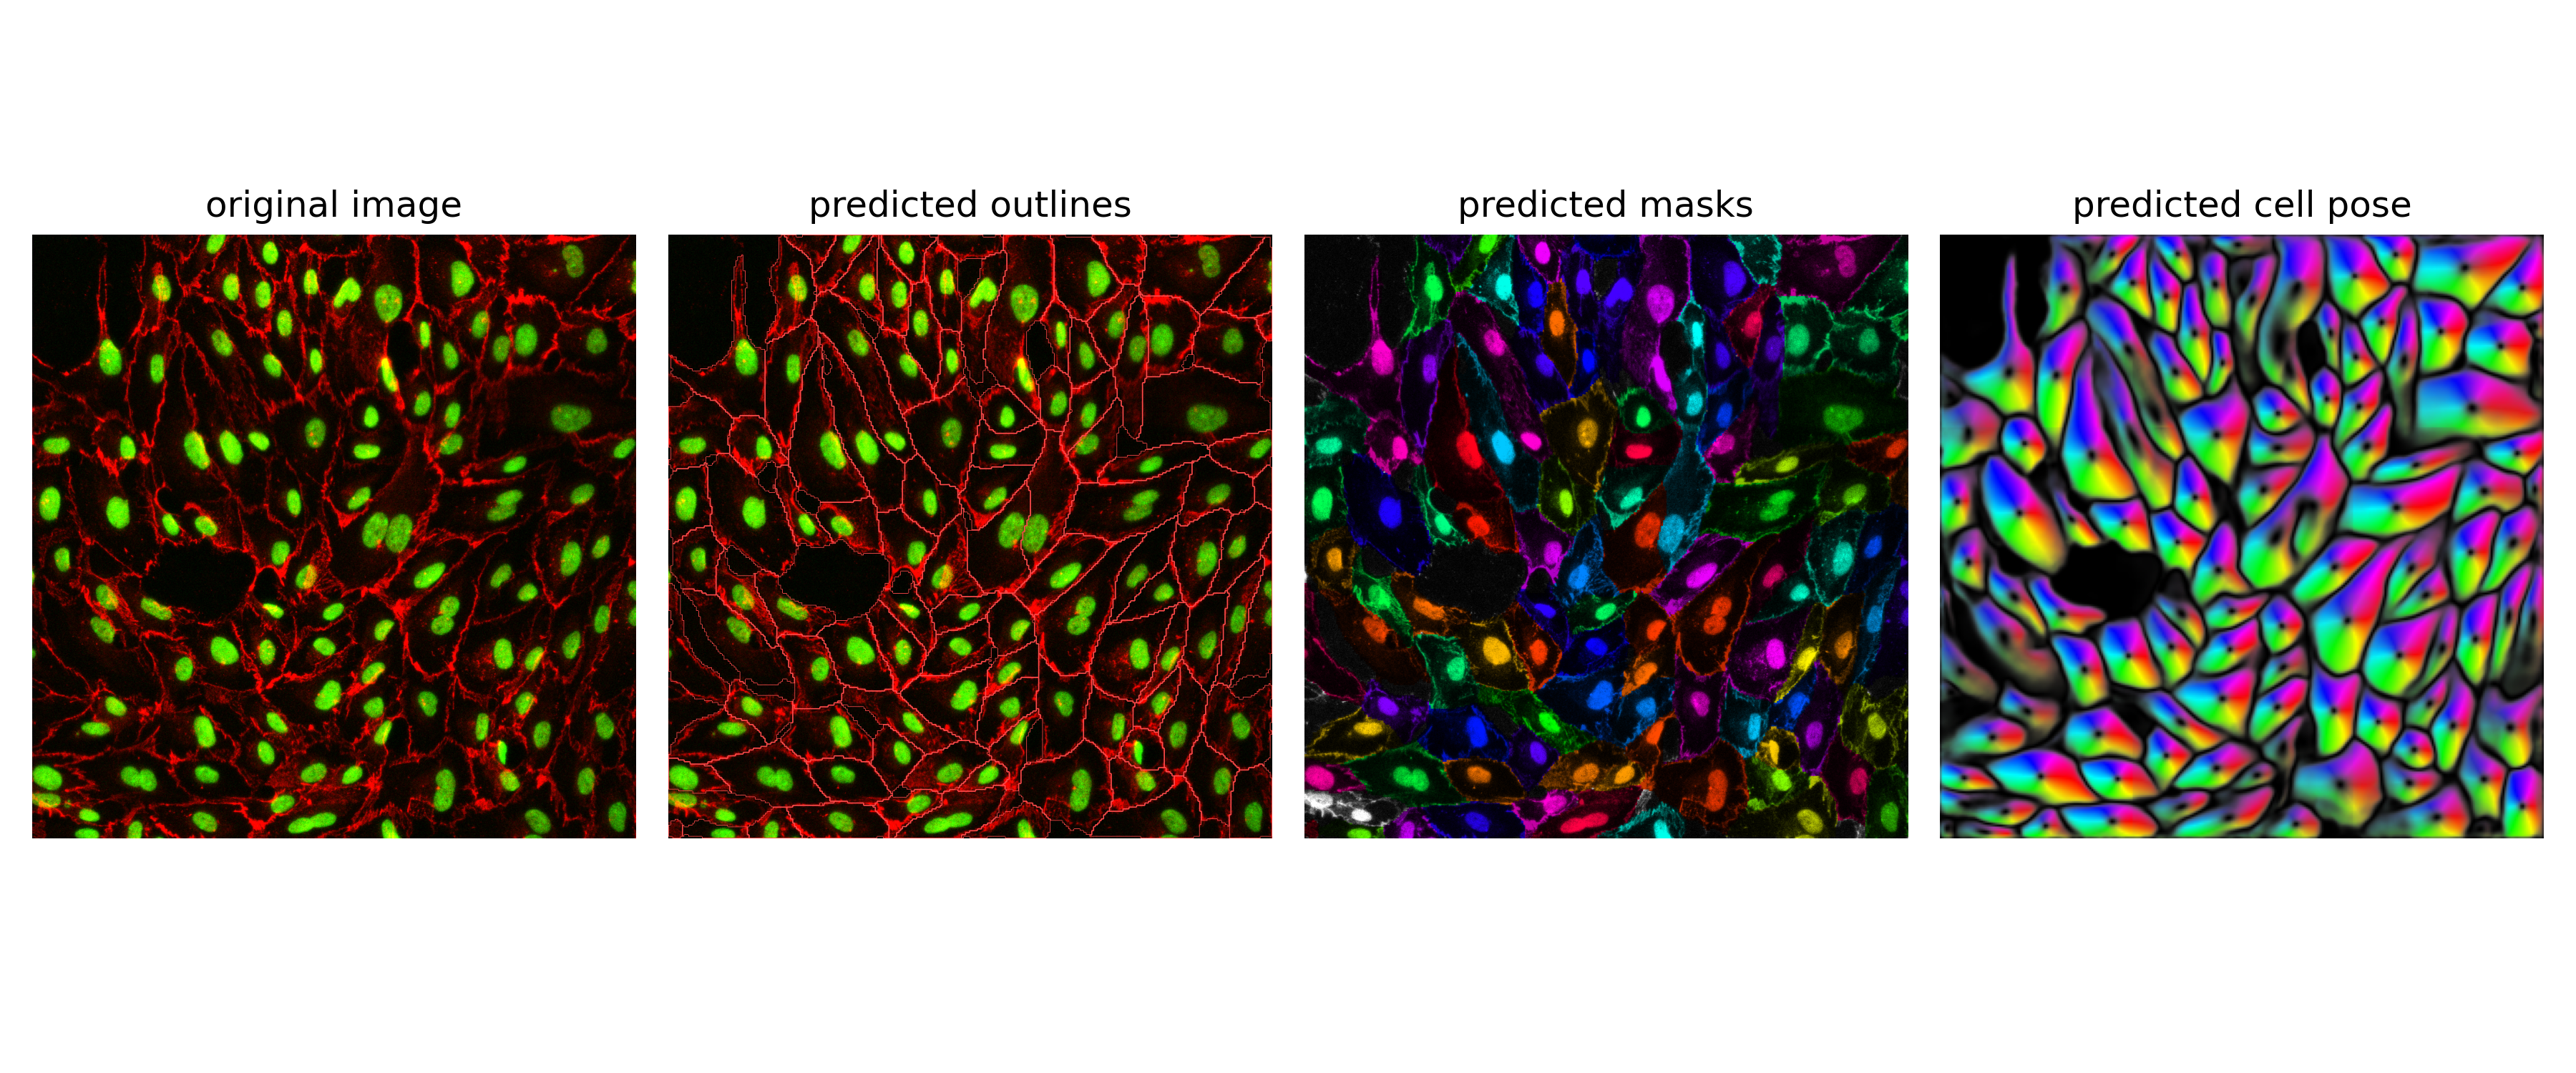
\includegraphics[width=1.0\textwidth]{images/segmentation-example.png}\\
  \tiny
  Example: segmentation of endothelial cells exposed to flow.
\end{figure}


We use the deep learning algorithm Cellpose for endothelial cell segmentation based on junction and nuclei staining. Run python script with\\[0.5cm]
%\begin{verbatim}
    \texttt{python run.py parameters.yml} \\[0.5cm]
%\end{verbatim}
Here, paramters specifies input image, channel order and output folder.

\end{frame}

\begin{frame}[plain]
\frametitle{\normalsize \bf Segmentation with Cellpose}

\centering

\tiny
\begin{figure}
  \centering
  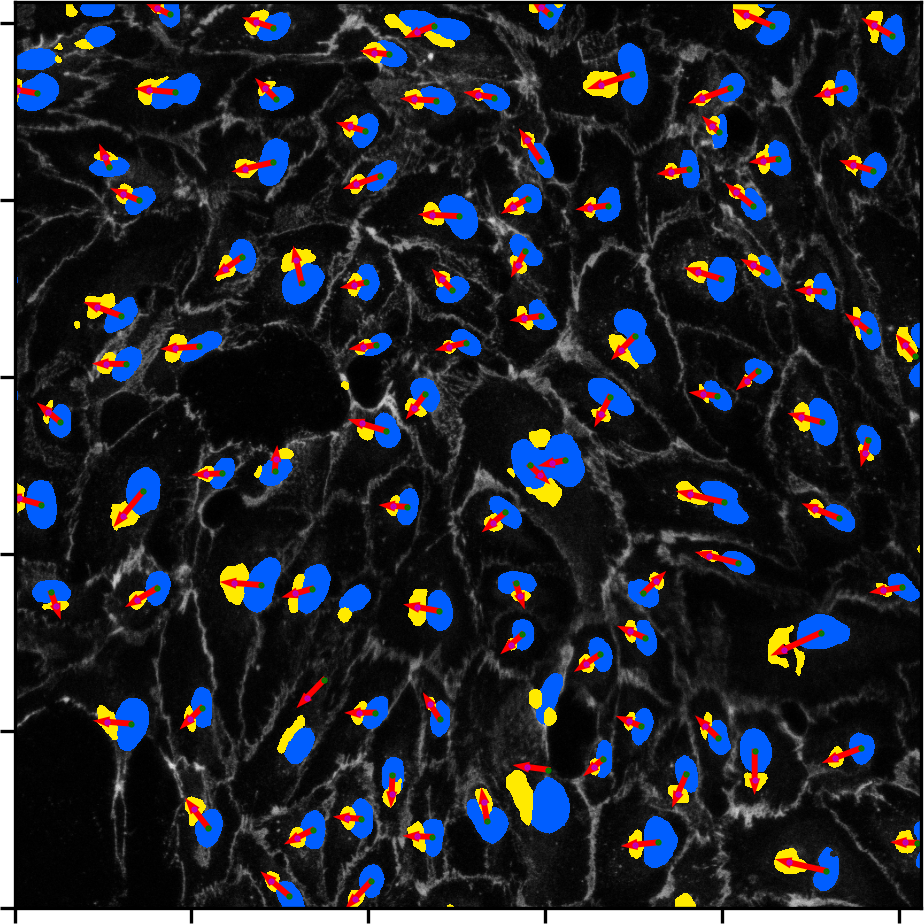
\includegraphics[width=0.7\textwidth]{images/image_001_nuclei_golgi_vector.png}\\
  \tiny
  Example: Automated segmentation of nuclei as well as golgi organelles and computation of nuclei-golgi vectors.
\end{figure}

\end{frame}



\begin{frame}[plain]
\frametitle{\normalsize \bf Segmentation with Cellpose}

\centering

\tiny
\begin{figure}
  \centering
  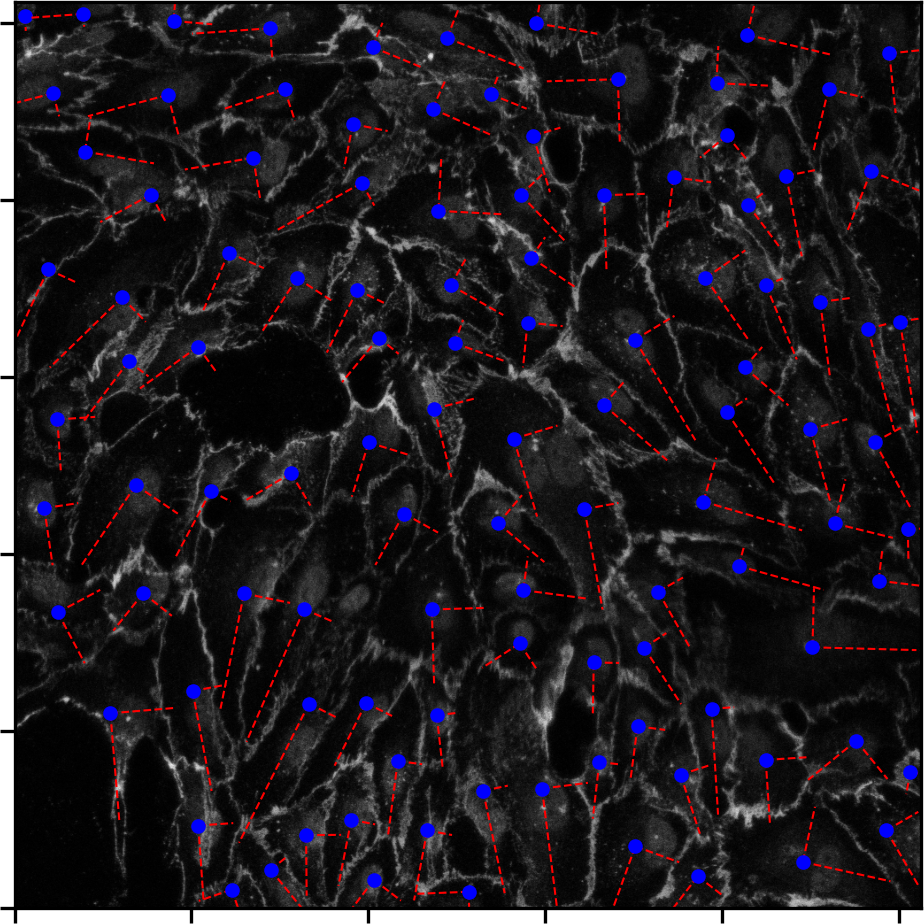
\includegraphics[width=0.7\textwidth]{images/image_001_cellshape_orientation.png}\\
  \tiny
  Computation of longest and shortest axis of cell shapes.
\end{figure}

\end{frame}





\begin{frame}
\frametitle{\normalsize \bf Polarity index}
\scriptsize
\centering

\begin{align}
    \text{Polarity index} = \sqrt{ \left(\frac{1}{N} \sum^N_{i=1} \cos \alpha_i \right)^2 + \left(\frac{1}{N} \sum^N_{i=1} \sin \alpha_i \right)^2}
\end{align}



\end{frame}


\begin{frame}
\frametitle{\normalsize \bf Signed polarity index}
\scriptsize
\centering

\begin{align}
    SPI = \frac{\text{\#cells against flow} - \text{\#cells with flow}}{\text{\#cells against flow} + \text{\#cells with flow}}
\end{align}



\end{frame}




%\plain{Thank you for your attention! Questions?}
\end{document}
